%\begin{savequote}[8cm]
%\textlatin{Cor animalium, fundamentum e\longs t vitæ, princeps omnium, Microco\longs mi Sol, a quo omnis vegetatio dependet, vigor omnis \& robur emanat.}
%
%The heart of animals is the foundation of their life, the sovereign of everything within them, the sun of their microcosm, that upon which all growth depends, from which all power proceeds.
%  \qauthor{--- William Harvey \cite{harvey_exercitatio_1628}}
%\end{savequote}

\chapter{\label{app:go-results}\label{app:expr-deets-ch4}Additional Experimental Details for Chapter 4}




\section{Grid world hyper-parameter search and additional results} 
\label{appsec:hps}

    \todo{This is copy and pasted from neurips at the moment. It doesn't account for the changes made to the algorithms or now using BayesOpt. Need to describe the parameter space searched over for each algorithm, how many Bayes trials were used and how each bayes tirla evaluated. And also give the final values used in tables. Manually setting Qinit function, but no prior knowledge used other than this.}

    To select hyper-parameters for the experiments detailed in Section \ref{sec:gridworlds}, we performed a hyper-parameter search. The search was run on the 8x12 Frozen Lake environment from Figure \ref{fig:fl12}, and the results in Section \ref{sec:gridworlds} were run on the 8x12 Frozen Lake envrionment from Figure \ref{fig:fl12test}. For the Sailing problem, we performed the search using an initial wind direction of North, and the result in Section \ref{sec:results} used an initial wind direction of South-East.

    To avoid the search space from becoming too large, we set some parameters manually. A good rule of thumb for initial values is to assure that $Q^{\text{init}}_{\text{sft}}(s,a) < Q_{\sft}^*(s,a)$ and $Q^{\text{init}}(s,a) < Q^*(s,a)$. Explicitly this means that an initial value of zero is \textit{not} a good choice for the Sailing problem, as rewards are negative (i.e. it has costs). In the Sailing environment, we actually set the initial values to $-200$, so that they were equal to the lowest possible return from a trial (the trial length was set to $50$, and an agent can incur a cost of at most $-4$ per timestep). To simplify the search space, we initially set the decay function in DENTS to $\beta(m)=\alpha/\log(e+m)$ and tune it after. 

    For the remaining parameters, we considered all combinations of the following values:
    \begin{itemize}
        \item \textit{UCT Bias}: \todo{cite}%\citeapp{prst}
            , 100.0, 10.0, 1.0, 0.1;
        \item \textit{MENTS exploration coefficient}: 2.0, 1.0, 0.3, 0.1, 0.03, 0.01;
        \item \textit{Temperature}: 100.0, 10.0, 1.0, 0.1, 0.01, 0.001;
        \item \textit{HMCTS UCT budget}: 100000, 30000, 10000, 3000, 1000, 300, 100, 30, 10.
    \end{itemize}

    Where a UCT bias of \todo{cite}%\citeapp{prst}
    refers to the adaptive bias introduced by Keller and Eyerich \todo{cite}%\citeapp{prst}
    , and `temperature' refers to the relevant temperature for the algorithm (i.e. search temperature in BTS and DENTS, and the temperature for Shannon/Relative/Tsallis entropy in MENTS/RENTS/DENTS). After that search, for DENTS we considered the decay functions of the form $\beta(m)=\beta_{\text{init}}/\log(e+m)$ and considered the following values:
    \begin{itemize}
            \item \textit{DENTS initial entropy temperature} ($\beta_{\text{init}}$): 100.0, 10.0, 1.0, 0.1.
    \end{itemize}
    The final set of hyperparameters is given in Tables \ref{table:hyper_fl} and \ref{table:hyper_s}, which were used in the gridworld experiments in Section \ref{sec:gridworlds}. Not included in the tables: \todo{cite}%\citeapp{prst}
    was selected for the UCT bias in both Frozen Lake and the Sailing problem.

    \begin{table}[]
        \centering
        \begin{tabular}{r|ccc} 
            Algorithm   & Exploration Parameter ($\epsilon$)    & Temperature ($\alpha$)    & Initial Values ($Q^{\text{init}}$, $Q^{\text{init}}_{\text{sft}}$)    \\
            \hline
            MENTS       & 1.0                                   & 0.001                     & 0                                                                     \\
            RENTS       & 2.0                                   & 0.001                     & 0                                                                     \\
            TENTS       & 1.0                                   & 0.001                     & 0                                                                     \\
            BTS         & 2.0                                   & 0.1                       & 0                                                                     \\
            DENTS       & 1.0                                   & 0.1                       & 0                                                                     \\
        \end{tabular}
        \caption[Final hyperparameters used for Frozen Lake in Section \ref{sec:gridworlds}]{Final hyperparameters used for Frozen Lake in Section \ref{sec:gridworlds}. Not included in the table: \todo{cite}%\citeapp{prst}
        was selected for the bias in UCT, \todo{cite}%\citeapp{prst}
        was selected for the bias and 3000 for the UCT budget in HMCTS and $\beta_{\text{init}}=1.0$ was selected as the initial entropy temperature for DENTS. \label{table:hyper_fl}}
    \end{table}

    \begin{table}[]
        \centering
        \begin{tabular}{r|ccc} 
            Algorithm   & Exploration Parameter ($\epsilon$)    & Temperature ($\alpha$)    & Initial Values ($Q^{\text{init}}$, $Q^{\text{init}}_{\text{sft}}$)    \\
            \hline
            MENTS       & 1.0                                   & 10.0                      & -200                                                                  \\
            RENTS       & 1.0                                   & 10.0                      & -200                                                                  \\
            TENTS       & 2.0                                   & 0.1                       & -200                                                                  \\
            BTS         & 1.0                                   & 10.0                      & -200                                                                  \\
            DENTS       & 1.0                                   & 10.0                      & -200                                                                  \\
        \end{tabular}
        \caption[Final hyperparameters used for the Sailing Problem in Section \ref{sec:gridworlds}]{Final hyperparameters used for the Sailing Problem in Section \ref{sec:gridworlds}. Not included in the table: \todo{cite}%\citeapp{prst}
        was selected for the bias in UCT, \todo{cite}%\citeapp{prst}
        was selected for the bias and 30 for the UCT budget in HMCTS and $\beta_{\text{init}}=10.0$ was selected as the initial entropy temperature for DENTS. \label{table:hyper_s}}
    \end{table}












\section{DENTS with a constant $\beta$} 
\label{appsec:dents_mimic_ments}

\htodo{this subsubsection currently just a c and p from neurips}

\todo{Place this better? Or maybe just remove from thesis?}

To empirically demonstrate that DENTS search policy can mimic the search policy of MENTS, we ran DENTS with $\alpha=1.0,\beta(m)=\alpha$ on the 10-chain environment, and compared it to MENTS with $\alpha=1.0$. We also ran DENTS with $\alpha=0.001, \beta(m)=\alpha$ in the Frozen Lake environment, and compared it to MENTS with $\alpha=0.001$ which is what was selected in the hpyerparameter search (Appendix \ref{app:hps}). Results are given in Figure \ref{fig:dbments}. Note that in the 10-chain, only MENTS has a dip in performance initially, which is due to the two algorithms using different recommendation policies.


\begin{figure*}
    \centering
    \begin{subfigure}[b]{0.49\textwidth}
        \centering
        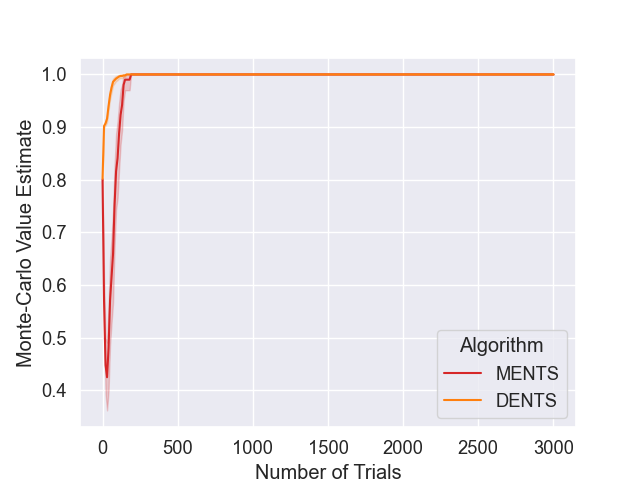
\includegraphics[width=\textwidth]{figures/temp/dbments/dbments_dchain.png}
        \caption{10-chain.}
    \end{subfigure}
    \begin{subfigure}[b]{0.49\textwidth}
        \centering
        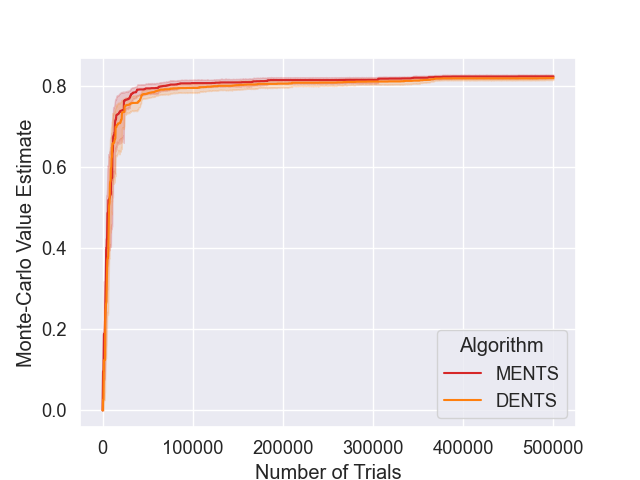
\includegraphics[width=\textwidth]{figures/temp/dbments/dbments_fl.png}
        \caption{Frozen Lake.}
    \end{subfigure}
    \caption{Comparing DENTS with MENTS, by setting $\beta_{\text{DENTS}}(m)=\alpha_{\text{MENTS}}, \alpha_{\text{DENTS}}=\alpha_{\text{MENTS}}$, where $\alpha_{\text{MENTS}}$ is the temperature used for MENTS, and $\alpha_{\text{DENTS}},\beta_{\text{DENTS}}$ are the temperatures used by DENTS.  \todo{Update fig?}}
    \label{fig:dbments}
\end{figure*}














\section{Additional Go details, results and discussion} 
\label{appsec:go_hps}
    \todo{Everything in this section this in this appendix is C and P from NeruIPS Go parameter tuning section.}

    \htodo{Just change the form of beta decay back to the inv sqrt used before. We tried lots of entropy things and nothing really worked.}

    Recall from Appendix \ref{app:adapt_for_games} that we initialised values with the neural networks as $Q^{\text{init}}(s,a)=\log \tilde{\pi}(a|s)+B$ and $V^{\text{init}}(s)=\tilde{V}(s)$, where $B$ is a constant (adapted from Xiao \todo{fixcites} %\etal \cite{xiao2019maximum}). 
    For these experiments we set a value of $B=\frac{-1}{|\mathcal{A}|}\sum_{a\in\mathcal{A}} \log\tilde{\pi}(a|s)$. Initialising the values in such a way tends to lead to the values of $Q^{\text{init}}(s,a)$ being in the range $[-20,20]$, to account for this, we scaled the results of the game to $100$ and $-100$, which means that any parameters selected are about $100$ times larger than they would be if we had not have used this scaling.
    
    In these experiments we used a recommendation policy that recommends the action that was sampled the most, i.e. $\psi(s)=\max_a N(s,a)$, as this tends to be more robust to any noise from neural network outputs.
    
    To select each parameter we ran a round robin tournament where we varied the value of one parameter. The agent that won the most games was used to select the parameter moving forward, and in the case of a tie we used the agent which won the most games. If the winning agent had the largest or smallest value, then we ran another tournament adjusting the values accordingly.
    
    We tuned all of these algorithms using the game of 9x9 Go with a komi of 6.5, and giving each algorithm 2.5 seconds per move. For our final results we used the same parameters on 19x19 Go with a komi of 7.5, giving each algorithm 5.0 seconds per move.






\subsection{Parameter selection for Go and supplimentary results} \label{app:go_hps}

    In this section we work through the process used to select parameters for the Go round robin tournament used in Section \ref{sec:go}. Predominantly parameters were chosen by playing out games of Go between agents. The parameters used for PUCT were copied from Kata Go and Alpha Go Zero \todo{fix cites} %\citeapp{katago,silver2017mastering}. 
    
    Initially we set the values of $\epsilon,\epsilon_{\tilde{\lambda}}$ to $0.03,1.0$. In Tables \ref{tab:w001} and \ref{tab:x001} we give results of tuning the search temperature for BTS and AR-BTS. For AR-BTS we tried different values of $\alpha_{\text{init}}$ in $\alpha(m)=\alpha_{\text{init}}/\sqrt{m}$.
    
    \begin{table*}[]
    \centering
        \begin{tabular}{l|cccccc}
            \textbf{Black \textbackslash White}     & 3  & 1   & 0.3   & 0.1    & 0.03    \\ 
            \hline
                                    3            & -     	& 7-8  		& 9-6  		&  12-3 		& 12-3  		\\
                                    1            & 15-0 & - & 12-3 & 15-0 & 15-0   		\\
                                    0.3          & 13-2 & 11-4 & - & 14-1 & 15-0  		\\
                                    0.1          & 14-1 & 10-5 & 11-4 & - & 15-0   		\\
                                    0.03         & 13-2 & 5-10 & 8-7 & 13-2 &   -   	\\    
        \end{tabular}
        \caption{Results for round robin to select the temperature parameter $\alpha$ for BTS. The value of 1.0 won all four of its matches so was selected. \label{tab:w001}}
    \end{table*}
    
    \begin{table*}[]
    \centering
        \begin{tabular}{l|cccccc}
            \textbf{Black \textbackslash White}     & 3  & 1   & 0.3   & 0.1    & 0.03    \\ 
            \hline
                                    3            & -     & 3-12  & 4-11  & 3-12  & 1-14  \\
                                    1             & 14-1  & -     & 8-7  & 9-6  & 7-8  \\
                                    0.3             & 14-1   & 8-7   &   -   & 7-8  & 11-4  \\
                                    0.1              & 15-0  & 11-4  & 9-6  & -     & 9-6  \\
                                    0.03              & 14-1  & 8-7  & 4-11  & 8-7  &   -   \\    
        \end{tabular}
        \caption{Results for round robin to select the temperature parameter $\alpha_{\text{init}}$ for AR-BTS. The value of 0.1 won all four of its matches so was selected. \label{tab:x001}}
    \end{table*}
    
    
    
    
    
    
    We then tuned the weighting of the prior policy $\epsilon_{\tilde{\lambda}}$. In Tables \ref{tab:w020} and \ref{tab:x020} we give results of tuning the prior policy weight for BTS and AR-BTS.
    
    \begin{table*}[]
    \centering
        \begin{tabular}{l|cccccc}
            \textbf{Black \textbackslash White}     & 10  & 5   & 3   & 2    & 1    \\ 
            \hline
                                    10            & - & 5-10 & 3-12 & 1-14 &  3-12  		\\
                                    5            & 14-1 & - & 12-3 & 11-4 & 11-4   		\\
                                    3          & 15-0 & 15-0 & - & 12-3 & 12-3   		\\
                                    2          & 15-0 & 12-3 & 12-3 & - & 10-5   		\\
                                    1         & 15-0 & 14-1 & 12-3 & 9-6 &   -   	\\    
        \end{tabular}
        \caption{Results for round robin to select the weighting of the prior policy $\epsilon_{\tilde{\lambda}}$ for BTS. The value of 2.0 won the most matches so was selected. \label{tab:w020}}
    \end{table*}
    
    \begin{table*}[]
    \centering
        \begin{tabular}{l|cccccc}
            \textbf{Black \textbackslash White}     & 3  & 2   & 1   & 0.75    & 0.5    \\ 
            \hline
                                    3            & - & 14-1 & 9-6 & 13-2 & 14-1   		\\
                                    2            & 12-3 & - & 12-3 & 15-0 & 10-5   		\\
                                    1          & 12-3 & 13-2 & - & 11-4 & 13-2   		\\
                                    0.75          & 11-4 & 10-5 & 12-3 & - & 14-1   		\\
                                    0.5         & 11-4 & 13-2 & 9-6 & 7-8 &   -   	\\   
        \end{tabular}
        \caption{Results for round robin to select the weighting of the prior policy $\epsilon_{\tilde{\lambda}}$ for AR-BTS. The value of 1.0 won the most matches so was selected. \label{tab:x020}}
    \end{table*}
    
    
    
    
    
    
    Following that, we then tuned MENTS exploration parameter $\epsilon$. In Tables \ref{tab:w030} and \ref{tab:x030} we give results of tuning the exploration parameter for BTS and AR-BTS. Although we selected the lowest value we tried here, we note that with such a value that a random action would have been sampled very few times, so the result of the hyperparameter selection was essentially that $\epsilon$ should be as low as possible.
    
    \begin{table*}[]
    \centering
        \begin{tabular}{l|cccccc}
            \textbf{Black \textbackslash White}     & 0.1  & 0.03   & 0.01   & 0.003    & 0.001    \\ 
            \hline
                                    0.1            & - & 12-3 & 10-5 & 8-7 & 7-8   		\\
                                    0.03            & 9-6 & - & 8-7 & 13-2 & 12-3   		\\
                                    0.01          & 11-4 & 9-6 & - & 7-8 & 12-3   		\\
                                    0.003          & 13-2 & 9-6 & 11-4 & - & 11-4   		\\
                                    0.001         & 12-3 & 11-4 & 8-7 & 9-6 &   -   	\\    
        \end{tabular}
        \caption{Results for round robin to select the exploration parameter $\epsilon$ for BTS. The value of 0.003 won the most matches so was selected. \label{tab:w030}}
    \end{table*}
    
    \begin{table*}[]
    \centering
        \begin{tabular}{l|cccccc}
            \textbf{Black \textbackslash White}     & 0.1  & 0.03   & 0.01   & 0.003    & 0.001    \\ 
            \hline
                                    0.1            & - & 12-3 & 14-1 & 12-3 & 13-2   		\\
                                    0.03            & 15-0 & - & 11-4 & 14-1 & 14-1   		\\
                                    0.01          & 15-0 & 11-4 & - & 13-2 & 13-2   		\\
                                    0.003          & 15-0 & 14-0 & 14-1 & - & 13-2   		\\
                                    0.001         & 14-1 & 14-1 & 14-1 & 15-0 &   -   	\\    
        \end{tabular}
        \caption{Results for round robin to select the exploration parameter $\epsilon$ for AR-BTS. The value of 0.001 won the most matches so was selected. \label{tab:x030}}
    \end{table*}
    
    
    
    
    
    
    
    
    
    Then we tuned the (fixed and constant) search temperatures for MENTS, AR-MENTS, RENTS, AR-RENTS, TENTS and AR-TENTS in tables \ref{tab:w040}, \ref{tab:x040},\ref{tab:w050}, \ref{tab:x050},\ref{tab:w060} and \ref{tab:x060}.
    
    
    
    
    \begin{table*}[]
    \centering
        \begin{tabular}{l|cccccc}
            \textbf{Black \textbackslash White}     & 3  & 1   & 0.3   & 0.1    & 0.03    \\ 
            \hline
                                    3            & -     	&   	9-6	&  9-6 		&   	11-4	&  10-5 		\\
                                    1            & 11-4  		& -     	&  11-4		&  9-6 		& 10-5  		\\
                                    0.3          &  9-6  	&  7-8  	&   -   &  11-4 		&  6-9 		\\
                                    0.1          &  4-11 		&   4-11		&   0-15		& -     	&  4-11 		\\
                                    0.03         &   	2-13	&  2-13 		&  0-15 		&   0-15		&   -   	\\      
        \end{tabular}
        \caption{Results for round robin to select the temperature parameter $\alpha$ for MENTS. The value of 1.0 won the most matches so was selected. \label{tab:w040}}
    \end{table*}
    
    \begin{table*}[]
    \centering
        \begin{tabular}{l|cccccc}
            \textbf{Black \textbackslash White}     & 3  & 1   & 0.3   & 0.1    & 0.03    \\ 
            \hline
                                    3            & -     	&  2-13 		& 1-14  		& 3-12  		& 5-10  		\\
                                    1            &  14-1 		& -     	& 11-4 		& 13-2  		& 15-0  		\\
                                    0.3          &  15-0  	&  12-3  	&   -   &  12-3 		& 14-1  		\\
                                    0.1          &   15-0		&  9-6 		&  9-6 		& -     	&  15-0 		\\
                                    0.03         &   15-0		&  8-7 		&  9-6 		& 14-1  		&   -   	\\    
        \end{tabular}
        \caption{Results for round robin to select the temperature parameter $\alpha$ for AR-MENTS. The value of 0.3 won the most matches so was selected. \label{tab:x040}}
    \end{table*}
    
    \begin{table*}[]
    \centering
        \begin{tabular}{l|cccccc}
            \textbf{Black \textbackslash White}     & 3  & 1   & 0.3   & 0.1    & 0.03    \\ 
            \hline
                                    3            & -     	&   	7-8	&  9-6 		&  10-5 		&  9-6 		\\
                                    1            &  13-2 		& -     	& 12-3 		& 11-4  		&  12-3 		\\
                                    0.3          &   10-5 	& 11-4   	&   -   &  10-5 		&  5-10 		\\
                                    0.1          &   3-12		&  2-13 		& 1-14  		& -     	&  3-12 		\\
                                    0.03         &   3-12		&  0-15 		&  0-15 		&  0-15 		&   -   	\\    
        \end{tabular}
        \caption{Results for round robin to select the temperature parameter $\alpha$ for RENTS. The value of 1.0 won the most matches so was selected. \label{tab:w050}}
    \end{table*}
    
    \begin{table*}[]
    \centering
        \begin{tabular}{l|cccccc}
            \textbf{Black \textbackslash White}     & 3  & 1   & 0.3   & 0.1    & 0.03    \\ 
            \hline
                                    3            & -     	&  4-11 		&  2-13 		& 9-6  		& 3-12  		\\
                                    1            &  15-0 		& -     	&  12-3		& 13-2  		&   13-2		\\
                                    0.3          &  15-0  	&  13-2  	&   -   &  14-1 		&  15-0 		\\
                                    0.1          &  15-0 		&   10-5		&   13-2		& -     	&  15-0 		\\
                                    0.03         &  13-2 		&  13-2 		&  12-3 		&   	14-1	&   -   	\\    
        \end{tabular}
        \caption{Results for round robin to select the temperature parameter $\alpha$ for AR-RENTS. The value of 0.3 won the most matches so was selected. \label{tab:x050}}
    \end{table*}
    
    \begin{table*}[]
    \centering
        \begin{tabular}{l|cccccc}
            \textbf{Black \textbackslash White}     & 300  & 100   & 30   & 10    & 3    \\ 
            \hline
                                    300            & -     	&  3-12 		&  5-10 		&  7-8 		& 9-6  		\\
                                    100            &  6-9 		& -     	&  9-6		&  12-3 		& 12-3  		\\
                                    30          & 8-7   	&  7-8  	&   -   &  9-6 		&  11-4 		\\
                                    10          &  0-15 		&  2-13 		& 2-13  		& -     	& 6-9  		\\
                                    3         &  1-14 		& 1-14  		& 2-13  		&  5-10 		&   -   	\\    
        \end{tabular}
        \caption{Results for round robin to select the temperature parameter $\alpha$ for TENTS. The value of 30.0 won the most matches so was selected. \label{tab:w060}}
    \end{table*}
    
    \begin{table*}[]
    \centering
        \begin{tabular}{l|cccccc}
            \textbf{Black \textbackslash White}     & 30  & 10   & 3   & 1    & 0.3    \\ 
            \hline
                                    30            & -     	&  14-1 		& 15-0  		& 14-1  		& 14-1  		\\
                                    10            &  15-0 		& -     	&  13-2		& 15-0  		&  15-0 		\\
                                    3          &  15-0  	&   14-1 	&   -   &  14-1 		&  15-0 		\\
                                    1          &   	15-0	&  15-0 		&  14-1 		& -     	& 15-0  		\\
                                    0.3         &   15-0		&   	15-0	&   14-1		& 15-0  		&   -   	\\    
        \end{tabular}
        \caption{Results for round robin to select the temperature parameter $\alpha$ for AR-TENTS. The value of 3.0 won the most matches so was selected. \label{tab:x060}}
    \end{table*}
    
    
    
    
    
    
    
    
    
    
    Finally, we considered entropy temperatures of the form $\beta(m)=\beta_{\text{init}}\frac{1+\exp(-5)}{1+\exp(m-5)}$ for DENTS and AR-DENTS, and tuned the value of $\beta_{\text{init}}$, in Tables \ref{tab:w070} and \ref{tab:x070} for DENTS and AR-DENTS respectively.
    
    
    \begin{table*}[]
    \centering
        \begin{tabular}{l|cccccc}
            \textbf{Black \textbackslash White}     & 0.1  & 0.03   & 0.01   & 0.003    & 0.001    \\ 
            \hline
                                    0.1            & - & 10-5 & 12-3 & 8-7 & 11-4  		\\
                                    0.03            & 13-2 & - & 11-4 & 13-2  & 10-5   		\\
                                    0.01            & 12-3 & 11-4 & - & 10-5 & 11-4  		\\
                                    0.003            & 7-8 & 13-2 & 13-2 & - & 10-5  		\\
                                    0.001           & 13-2 & 13-2 & 11-4 & 11-4 &  - 		\\
        \end{tabular}
        \caption{Results for round robin to select the initial entropy temperature $\beta_{\text{init}}$ for DENTS. The value of 0.3 won the most matches so was selected. \label{tab:w070}}
    \end{table*}
    
    \begin{table*}[]
    \centering
        \begin{tabular}{l|cccccc}
            \textbf{Black \textbackslash White}     & 3  & 1   & 0.3   & 0.1    & 0.03    \\ 
            \hline
                                    3            & - & 11-4 & 12-3 & 12-3 & 14-1  		\\
                                    1            & 13-2 & - & 11-4 & 13-2 & 13-2  		\\
                                    0.3            & 14-1 & 13-2 & - & 13-2 & 14-1  		\\
                                    0.1            & 12-3 & 12-3 & 12-3 & - & 11-4  		\\
                                    0.03            & 12-3 & 13-2 & 13-2 & 14-1 &  - 		\\
        \end{tabular}
        \caption{Results for round robin to select the initial entropy temperature $\beta_{\text{init}}$ for AR-DENTS. The value of 0.3 won the most matches so was selected. \label{tab:x070}}
    \end{table*}
    
    
    
    
    
    
    
    After tuning all of the algorithms, we compared each algorithm to their AR version in table \ref{tab:y10}, and the AR versions universally outperformed their counterparts. We used all of the selected parameters in 19x19 Go to run our final experiments given in Table \ref{table:go_results}.
    
    
    
    \begin{table*}[]
    \centering
        \begin{tabular}{l|cccccc}
            \textbf{Black \textbackslash White}     & MENTS     & AR-MENTS  & BTS       & AR-BTS    & DENTS     & AR-DENTS  \\ 
            \hline
                                    MENTS           &   -       & 0-25      &           &           &           &           \\
                                    AR-MENTS        & 25-0      &   -       &           &           &           &           \\
                                    BTS             &           &           &   -       & 16-9      &           &           \\
                                    AR-BTS          &           &           & 22-3      &   -       &           &           \\
                                    DENTS           &           &           &           &           &   -       & 21-4      \\
                                    AR-DENTS        &           &           &           &           & 22-3      & -         \\      
            \hline
            \textbf{Black \textbackslash White}     & RENTS     & AR-RENTS  & TENTS     & AR-TENTS  &           &           \\ 
            \hline
                                    RENTS           &   -       & 2-23      &           &           &           &           \\
                                    AR-RENTS        & 24-1      &   -       &           &           &           &           \\
                                    TENTS           &           &           &   -       & 8-17      &           &           \\
                                    AR-TENTS        &           &           & 23-2      & -         &           &           \\         
        \end{tabular}
        \caption{Results for the matches of each algorithm against its AR version.\label{tab:y10}}
    \end{table*}
    
    
    
    Finally, we also ran AR-BTS against Kata Go directly limiting each algorithm to 1600 trials. KataGo beat AR-BTS by 31-19, confirming that the aditional exploration is outweighed by the information contained in the neural networks, and in Go the Boltzmann search algorithms gain their advantage via the Alias method and being able to run more trials quickly.


